\documentclass[14pt]{extbook}
\usepackage{multicol, enumerate, enumitem, hyperref, color, soul, setspace, parskip, fancyhdr} %General Packages
\usepackage{amssymb, amsthm, amsmath, latexsym, units, mathtools} %Math Packages
\everymath{\displaystyle} %All math in Display Style
% Packages with additional options
\usepackage[headsep=0.5cm,headheight=12pt, left=1 in,right= 1 in,top= 1 in,bottom= 1 in]{geometry}
\usepackage[usenames,dvipsnames]{xcolor}
\usepackage{dashrule}  % Package to use the command below to create lines between items
\newcommand{\litem}[1]{\item#1\hspace*{-1cm}\rule{\textwidth}{0.4pt}}
\pagestyle{fancy}
\lhead{Progress Quiz 3}
\chead{}
\rhead{Version C}
\lfoot{3012-8528}
\cfoot{}
\rfoot{Summer C 2021}
\begin{document}

\begin{enumerate}
\litem{
Solve the quadratic equation below. Then, choose the intervals that the solutions belong to, with $x_1 \leq x_2$ (if they exist).\[ -16x^{2} -15 x + 8 = 0 \]\begin{enumerate}[label=\Alph*.]
\item \( x_1 \in [-0.8, 0.6] \text{ and } x_2 \in [0.5, 2.9] \)
\item \( x_1 \in [-6.5, -5.4] \text{ and } x_2 \in [20.4, 23.1] \)
\item \( x_1 \in [-28.9, -26.1] \text{ and } x_2 \in [25.8, 28.3] \)
\item \( x_1 \in [-1.4, -1.2] \text{ and } x_2 \in [-0.1, 0.8] \)
\item \( \text{There are no Real solutions.} \)

\end{enumerate} }
\litem{
Factor the quadratic below. Then, choose the intervals that contain the constants in the form $(ax+b)(cx+d); b \leq d.$\[ 54x^{2} -69 x + 20 \]\begin{enumerate}[label=\Alph*.]
\item \( a \in [1.1, 2.9], \hspace*{5mm} b \in [-8, 1], \hspace*{5mm} c \in [26.7, 27.1], \text{ and } \hspace*{5mm} d \in [-5, 6] \)
\item \( a \in [4.8, 7.1], \hspace*{5mm} b \in [-8, 1], \hspace*{5mm} c \in [7, 10.5], \text{ and } \hspace*{5mm} d \in [-5, 6] \)
\item \( a \in [16.5, 18.1], \hspace*{5mm} b \in [-8, 1], \hspace*{5mm} c \in [2.1, 4.6], \text{ and } \hspace*{5mm} d \in [-5, 6] \)
\item \( a \in [-1, 1.9], \hspace*{5mm} b \in [-49, -44], \hspace*{5mm} c \in [-1.6, 1.9], \text{ and } \hspace*{5mm} d \in [-26, -22] \)
\item \( \text{None of the above.} \)

\end{enumerate} }
\litem{
Solve the quadratic equation below. Then, choose the intervals that the solutions $x_1$ and $x_2$ belong to, with $x_1 \leq x_2$.\[ 20x^{2} +21 x -54 = 0 \]\begin{enumerate}[label=\Alph*.]
\item \( x_1 \in [-45.86, -43.9] \text{ and } x_2 \in [24, 24.04] \)
\item \( x_1 \in [-2.93, -1.16] \text{ and } x_2 \in [1.15, 1.23] \)
\item \( x_1 \in [-9.52, -7.6] \text{ and } x_2 \in [0.23, 0.33] \)
\item \( x_1 \in [-7.78, -6.38] \text{ and } x_2 \in [0.32, 0.43] \)
\item \( x_1 \in [-1.46, 0.27] \text{ and } x_2 \in [2.34, 2.49] \)

\end{enumerate} }
\litem{
Write the equation of the graph presented below in the form $f(x)=ax^2+bx+c$, assuming  $a=1$ or $a=-1$. Then, choose the intervals that $a, b,$ and $c$ belong to.
\begin{center}
    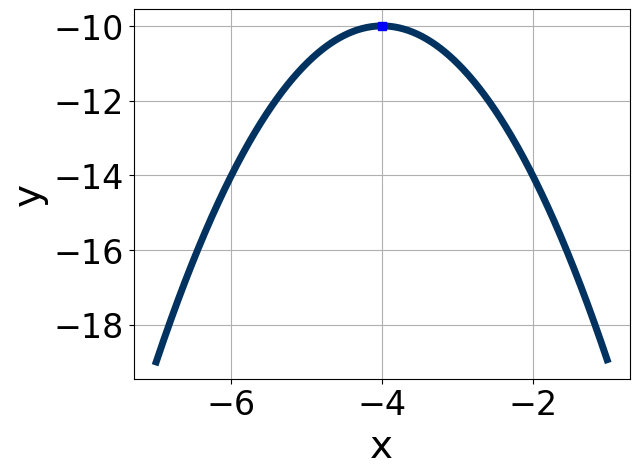
\includegraphics[width=0.5\textwidth]{../Figures/quadraticGraphToEquationCopyC.png}
\end{center}
\begin{enumerate}[label=\Alph*.]
\item \( a \in [-2.3, 0], \hspace*{5mm} b \in [7, 9], \text{ and } \hspace*{5mm} c \in [-29, -23] \)
\item \( a \in [-2.3, 0], \hspace*{5mm} b \in [-8, -5], \text{ and } \hspace*{5mm} c \in [-29, -23] \)
\item \( a \in [-0.8, 2], \hspace*{5mm} b \in [7, 9], \text{ and } \hspace*{5mm} c \in [5, 7] \)
\item \( a \in [-0.8, 2], \hspace*{5mm} b \in [-8, -5], \text{ and } \hspace*{5mm} c \in [5, 7] \)
\item \( a \in [-2.3, 0], \hspace*{5mm} b \in [7, 9], \text{ and } \hspace*{5mm} c \in [-9, 0] \)

\end{enumerate} }
\litem{
Graph the equation below.\[ f(x) = -(x-4)^2 - 20 \]\begin{enumerate}[label=\Alph*.]
\begin{multicols}{2}\item 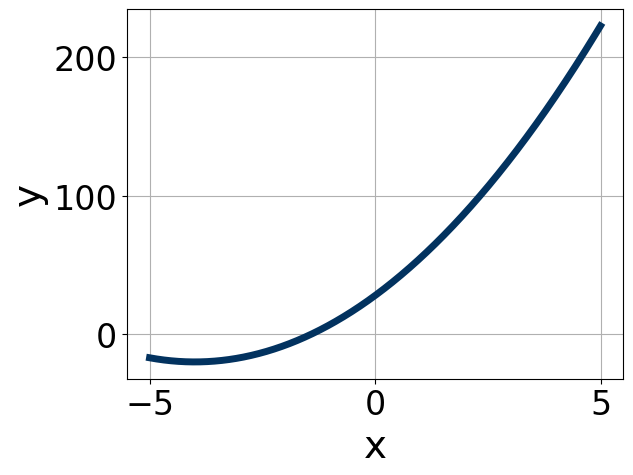
\includegraphics[width = 0.3\textwidth]{../Figures/quadraticEquationToGraphAC.png}\item 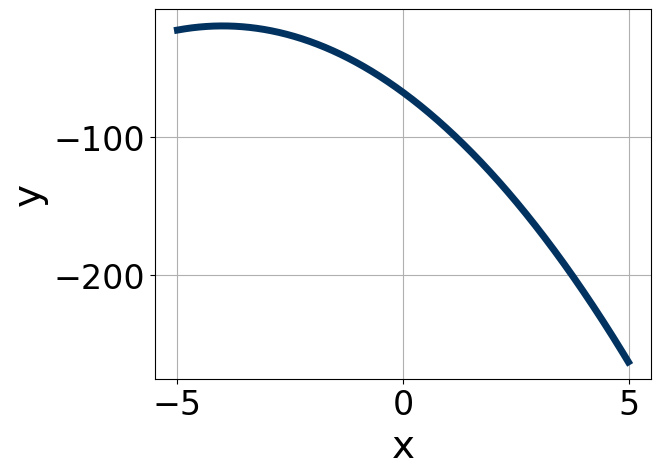
\includegraphics[width = 0.3\textwidth]{../Figures/quadraticEquationToGraphBC.png}\item 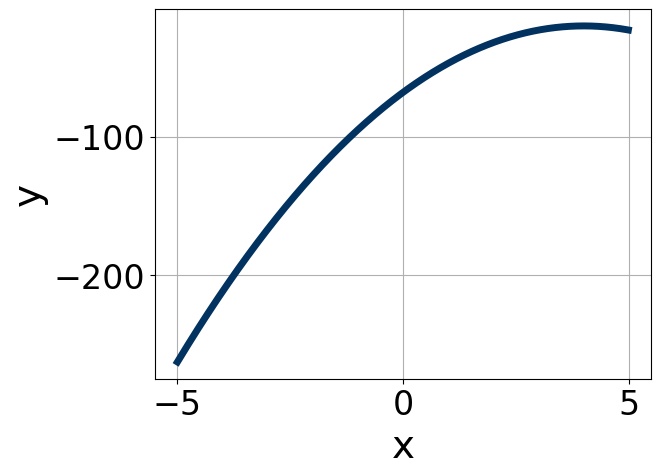
\includegraphics[width = 0.3\textwidth]{../Figures/quadraticEquationToGraphCC.png}\item 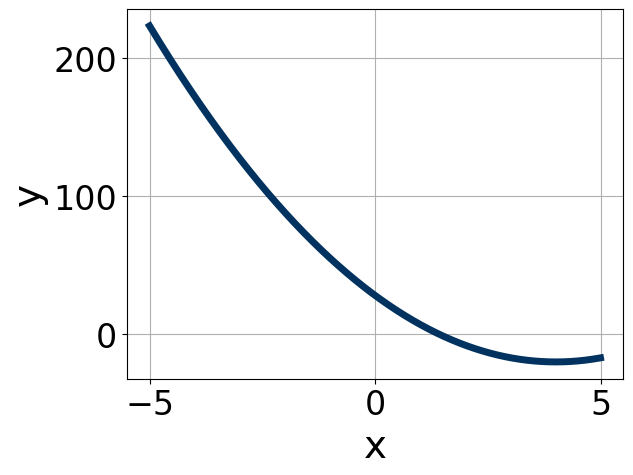
\includegraphics[width = 0.3\textwidth]{../Figures/quadraticEquationToGraphDC.png}\end{multicols}\item None of the above.
\end{enumerate} }
\litem{
Solve the quadratic equation below. Then, choose the intervals that the solutions $x_1$ and $x_2$ belong to, with $x_1 \leq x_2$.\[ 15x^{2} -38 x + 24 = 0 \]\begin{enumerate}[label=\Alph*.]
\item \( x_1 \in [17.89, 18.1] \text{ and } x_2 \in [19.88, 20.11] \)
\item \( x_1 \in [0.34, 0.59] \text{ and } x_2 \in [3.67, 4.24] \)
\item \( x_1 \in [1.15, 1.44] \text{ and } x_2 \in [1.18, 1.44] \)
\item \( x_1 \in [0.55, 0.63] \text{ and } x_2 \in [2.51, 2.95] \)
\item \( x_1 \in [0.66, 0.89] \text{ and } x_2 \in [2.33, 2.46] \)

\end{enumerate} }
\litem{
Factor the quadratic below. Then, choose the intervals that contain the constants in the form $(ax+b)(cx+d); b \leq d.$\[ 24x^{2} +38 x + 15 \]\begin{enumerate}[label=\Alph*.]
\item \( a \in [2.83, 5.18], \hspace*{5mm} b \in [-4, 5], \hspace*{5mm} c \in [5.75, 6.63], \text{ and } \hspace*{5mm} d \in [4, 6] \)
\item \( a \in [0.48, 1.02], \hspace*{5mm} b \in [14, 25], \hspace*{5mm} c \in [-0.66, 1.05], \text{ and } \hspace*{5mm} d \in [17, 21] \)
\item \( a \in [7.83, 8.35], \hspace*{5mm} b \in [-4, 5], \hspace*{5mm} c \in [2.9, 3.37], \text{ and } \hspace*{5mm} d \in [4, 6] \)
\item \( a \in [1.49, 2.68], \hspace*{5mm} b \in [-4, 5], \hspace*{5mm} c \in [10.76, 12.3], \text{ and } \hspace*{5mm} d \in [4, 6] \)
\item \( \text{None of the above.} \)

\end{enumerate} }
\litem{
Graph the equation below.\[ f(x) = -(x-4)^2 + 15 \]\begin{enumerate}[label=\Alph*.]
\begin{multicols}{2}\item 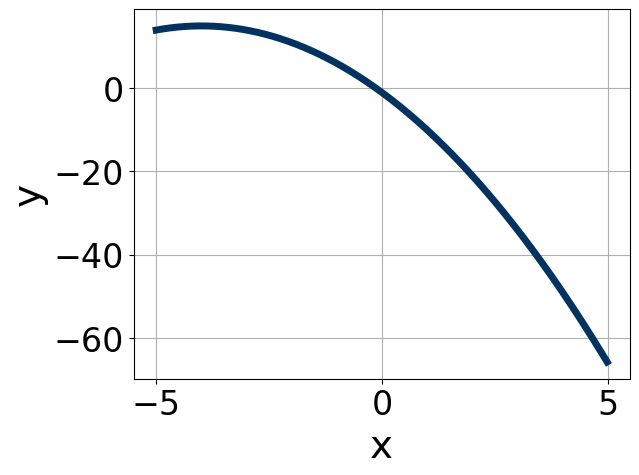
\includegraphics[width = 0.3\textwidth]{../Figures/quadraticEquationToGraphCopyAC.png}\item 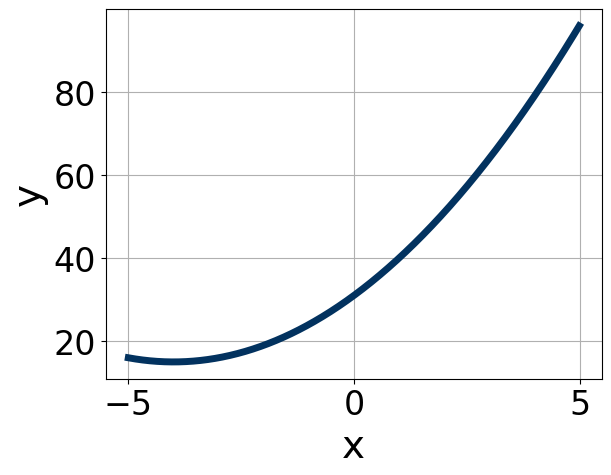
\includegraphics[width = 0.3\textwidth]{../Figures/quadraticEquationToGraphCopyBC.png}\item 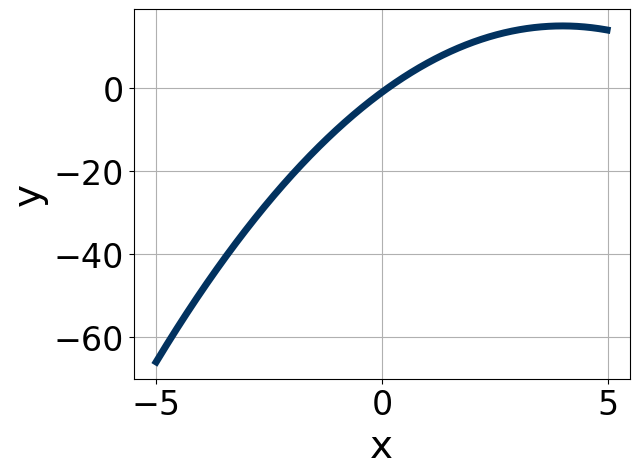
\includegraphics[width = 0.3\textwidth]{../Figures/quadraticEquationToGraphCopyCC.png}\item 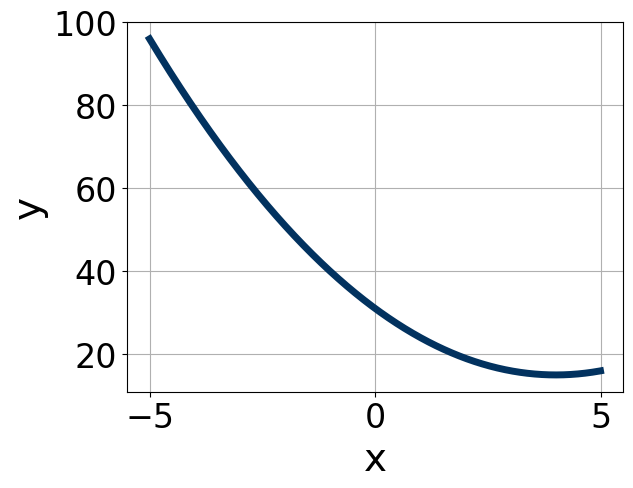
\includegraphics[width = 0.3\textwidth]{../Figures/quadraticEquationToGraphCopyDC.png}\end{multicols}\item None of the above.
\end{enumerate} }
\litem{
Solve the quadratic equation below. Then, choose the intervals that the solutions belong to, with $x_1 \leq x_2$ (if they exist).\[ 18x^{2} -9 x -6 = 0 \]\begin{enumerate}[label=\Alph*.]
\item \( x_1 \in [-1.49, -0.48] \text{ and } x_2 \in [-0.1, 0.46] \)
\item \( x_1 \in [-0.48, -0.37] \text{ and } x_2 \in [0.41, 1.42] \)
\item \( x_1 \in [-7.54, -6.59] \text{ and } x_2 \in [15.45, 16.28] \)
\item \( x_1 \in [-22.45, -21.84] \text{ and } x_2 \in [22.52, 23.78] \)
\item \( \text{There are no Real solutions.} \)

\end{enumerate} }
\litem{
Write the equation of the graph presented below in the form $f(x)=ax^2+bx+c$, assuming  $a=1$ or $a=-1$. Then, choose the intervals that $a, b,$ and $c$ belong to.
\begin{center}
    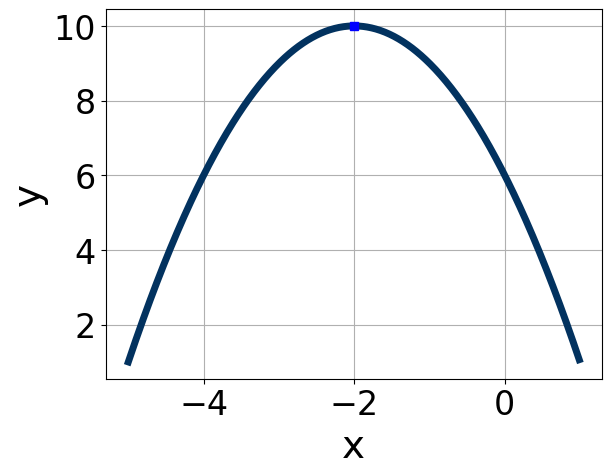
\includegraphics[width=0.5\textwidth]{../Figures/quadraticGraphToEquationC.png}
\end{center}
\begin{enumerate}[label=\Alph*.]
\item \( a \in [-1.1, -0.4], \hspace*{5mm} b \in [3, 6], \text{ and } \hspace*{5mm} c \in [-15, -10] \)
\item \( a \in [0.8, 2.9], \hspace*{5mm} b \in [3, 6], \text{ and } \hspace*{5mm} c \in [10, 15] \)
\item \( a \in [0.8, 2.9], \hspace*{5mm} b \in [-4, -1], \text{ and } \hspace*{5mm} c \in [10, 15] \)
\item \( a \in [-1.1, -0.4], \hspace*{5mm} b \in [-4, -1], \text{ and } \hspace*{5mm} c \in [4, 7] \)
\item \( a \in [-1.1, -0.4], \hspace*{5mm} b \in [3, 6], \text{ and } \hspace*{5mm} c \in [4, 7] \)

\end{enumerate} }
\end{enumerate}

\end{document}